%  Typ dokumentu - článek, prezentace aj.
\documentclass[english]{article}

%  Nastaví vstupní a výstupní kódování znaků (encoding) a lokalizace
\usepackage[T1]{fontenc}
\usepackage[utf8]{inputenc}
\usepackage[english,czech]{babel}
\usepackage{icomma}

%  Formát papíru a odsazení od jeho okrajů
\usepackage[letterpaper]{geometry}
\geometry{verbose,tmargin=1.5cm,bmargin=2cm,lmargin=2cm,rmargin=2cm}

%  Umožňuje pracovat s grafikou
\usepackage{graphicx}
\usepackage{bigstrut}
\usepackage{epstopdf}

%  Automaticky odsadí i první paragraf v každé sekci
\usepackage{indentfirst}

%  Umožňuje rozdělovat obsah na více sloupců
\usepackage{multicol}
\usepackage{booktabs}
\usepackage{pgffor}

%  Umožňuje používat hypertextové odkazy, nastavuje jejich barvu a
%  vlastnosti
\usepackage[unicode]{hyperref}
\hypersetup{
colorlinks=true, citecolor=blue, filecolor=blue, linkcolor=blue,
urlcolor=blue
}

%  Umožnění odstranění italiky u jednotek
\newcommand{\unit}[1]{\mathrm{#1}}

%  Formátování stránek, empty = odstraní číslování
% \pagestyle{empty}

%  Řádkování
\linespread{1.2}

%  Lepší zobrazování matematiky (rozšíření sum o \limits atd.)
\everymath{\displaystyle}
\usepackage{amsmath, amsthm, amssymb}

% Umožní psát přes \mathbb{N/R/Q/..} množiny čísel
\usepackage{amssymb}

%  Velikost fontu matematických výrazů v dokumentu lze pro danou
% základního fontu dokumentu upravit pomocí:
% \DeclareMathSizes{X}{Y}{Z}{U} kde:
% X je velikost fontu v dokumentu, pro kterou se matematika upraví
% Y je standartní velikost fontu matematiky
% Z je velikost fontu zmenšených (vnořených výrazů)
% U je velikost fontu ještě více zmenšených (vnořených výrazů).
\DeclareMathSizes{10}{10.5}{9}{9}

%  Nastaví autora, název, datum, skupinu měření apod. (můj vlastní
% příkaz, umožní znovu-použití v dokumentu)
\newcommand{\Author}{David Roesel}
\newcommand{\Coauthor}{Tereza Schönfeldová}
\newcommand{\Institute}{FJFI ČVUT v Praze}
\newcommand{\Subject}{FYZIKÁLNÍ PRAKTIKUM II}
\newcommand{\Group}{7}
\newcommand{\Circle}{ZS 7}
\newcommand{\Title}{Úloha \#12  \\Měření měrného náboje elektronu}
\newcommand{\Date}{31.3.2014}

% Začátek dokumentu - Formátování na výstup
\begin{document}

% Interní proměnné, možno zobrazovat u prezentací, používají se při
% generování pomocí \titlepage apod.
\author{\Author}
\title{\Title}
\date{\Date}

%  Lokalizace některých názvů do češtiny
\renewcommand{\figurename}{Obr.}
\renewcommand{\tablename}{Tab.}
\renewcommand{\refname}{Reference}

% --- Hlavička dokumentu -----------------------------------------------

\setlength{\parindent}{0cm}
\begin{multicols}{2}
\textbf{\Subject \\
        \Institute \\[0.1cm]
%\large  \Title \\[0.5cm]
\Title \\[0.5cm]
}
\begin{tabular}{rlrl}
\large Datum měření: & \Date & \large Skupina: & \Group \\
\large Jméno: & \Author & \large Kroužek:  & \Circle\\
\large Spolupracovala: & \Coauthor &\large Klasifikace:\\
\end{tabular}

\begin{flushright}

\includegraphics[scale=0.28]{../../_meta/fjfi_standart.pdf}
\hspace{0.2cm}
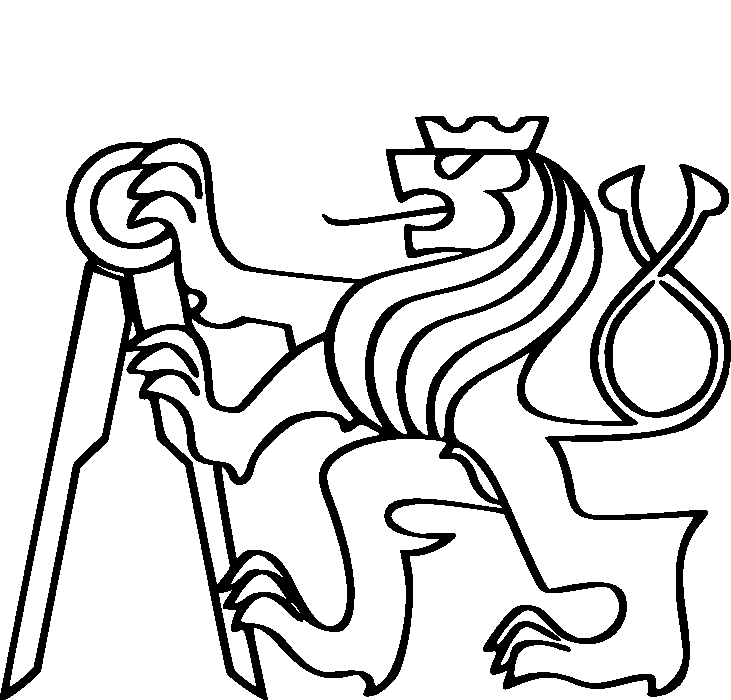
\includegraphics[scale=0.28]{../../_meta/cvut_standart.pdf}
\end{flushright}
\end{multicols}
\hrule
\vspace{0.5cm}

% ----------------------------------------------------------------------


% --- Tělo dokumentu ---------------------------------------------------
\setlength{\parindent}{0.5cm}
\section{Pracovní úkoly}
\begin{enumerate}
	\item Sestavte úlohu pro měření $e/m$ fokusací podélným magnetickým polem a proveďte měření pro čtyři různé hodnoty urychlovacího napětí $U$ v rozmezí 950~--~1250~V. Pomocné napětí na $A_1$ (viz Obr. \ref{fig:obrazek}) volte 140~V.
	\item Změřte měrný náboj elektronu $e/m$ ze zakřivení dráhy elektronů v kolmém magnetickém poli. Měření proveďte pro pět dvojic urychlovacího napětí a magnetizačního proudu. Vypočtěte příslušné hodnoty měrného náboje a z nich určete střední hodnotu.\\
	Doporučené hodnoty $U$ a $I$ jsou: 120~V/1,5~A; 140~V/1,5~A; 160~V/2~A; 200~V/2~A.
	\item Několikrát pootočte katodovou trubicí sem a tam vůči magnetickému poli a sledujte změnu trajektorie proudu elektronů. Uvidíte, že z kruhového tvaru ($\vec{v}\perp\vec{B}$) přejde na šroubovitý ($\vec{v}\not\perp\vec{B}$) a nakonec v přímku ($\vec{v}\parallel\vec{B}$). Nakreslete pozorované trajektorie do protokolu. Použijte napětí $U = 150$ V a proud $I = 1,5$ A.
\end{enumerate}

\section{Vypracování}

	\subsection{Použité přístroje}
		Zdroj napětí 300~V a 2~kV, zdroj proudu, katodová trubice firmy Leybold-Heraeus, Helmholtzovy cívky, ampérmetr, voltmetr, obrazovka s cívkou, propojovací vodiče, aparatura na měření průměrů drah elektronů v katodové trubici, zrcadlo, dřevěná posuvná měřítka, zástěna, zdroj proudu z úlohy 2.
		
	\subsection{Teoretický úvod}
		Poměr náboje elektronu $e$ k jeho hmotnosti $m$ nazýváme \emph{měrný náboj elektronu}. V soustavě SI má rozměr C/kg. K dispozici máme dvě metody na jeho změření: fokusací svazku v podélném magnetickém poli a sledováním zakřivení dráhy v magnetickém poli příčném. Základem obou metod je Lorentzova síla, která působí na každou nabitou částici (například elektron), která se pohybuje rychlostí $\vec{v}$ v magnetickém poli o vektoru magnetické indukce $\vec{B}$. Pro tuto sílu platí
		\begin{equation} \label{eq:lorentzova_sila}
		\vec{F} = e \left( \vec{v} \times \vec{B} \right).
		\end{equation}
		
		\subsubsection{Měření $e/m$ v podélném magnetickém poli}
			Jedná se o metodu založenou na působení podélného magnetického pole na divergující svazek elektronů, které vychází po urychlení z malého otvoru v anodě obrazovky osciloskopu. Vektor rychlosti elektronu $\vec{v}$ můžeme rozložit na dvě složky: kolmou $\vec{v}_{\perp}$ a podélnou $\vec{v}_{\parallel}$ (vzhledem ke směru magnetického pole). Pokud označíme $\alpha$ úhel mezi touto rychlostí a směrem vektoru $\vec{B}$, bude platit
			\begin{equation}
			\vec{v}_{\parallel} = v \cos \alpha, \qquad \vec{v}_{\perp} = v \sin \alpha.
			\end{equation}
			Vztah (\ref{eq:lorentzova_sila}) se pak nechá převést na tvar
			\begin{equation}
			\vec{F} = \vec{F}_{\perp} + \vec{F}_{\parallel} = e \left( \vec{v}_{\perp} \times \vec{B} \right) + e \underbrace{\left( \vec{v}_{\parallel} \times \vec{B} \right)}_{ (\vec{v}_{\parallel}\parallel\vec{B})\Rightarrow =0},
			\end{equation}
			přičemž poslední člen je vzhledem k rovnoběžnosti nulový. Magnetické pole působí na elektrony určitou silou a ta je kolmá na $\vec{v}_{\perp}$ i $\vec{B}$. Její velikost je rovna $e v_{\perp} B$. Vzhledem k tomu, že velikost rychlosti $\vec{v}_\perp$ zůstává konstantní, bude elektron opisovat kružnici. Tím pádem platí podmínka
			\begin{equation}
			e v_\perp B = \frac{m v_\perp^2}{r},
			\end{equation}
			ze které se dá vyjádřit úpravami
			\begin{equation}
			r = \frac{v_\perp}{\frac{e}{m} B} \qquad \qquad \text{a} \qquad \qquad v_\perp = \frac{e}{m} B r.
			\end{equation}
			
			Elektronu bude trvat opsat celou kružnici čas $T$, který určíme ze vztahu
			\begin{equation}
			T \frac{2 \pi r}{v_\perp} = \frac{2 \pi}{\frac{e}{m} B}.
			\end{equation}
			
			vzhledem k tomu, že elektrony současně vykonávají pohyb rychlostí $\vec{v}_\parallel$, bude výsledná dráha tvaru spirály. Rychlost $v_\parallel$ bude záviset na urychlovacím napětí $U$ a zároveň na rychlosti, kterou byly elektrony vyzařovány z katody. Dovolíme-li si zanedbat počáteční rychlost elektronů v porovnání s rychlostí po urychlení, bude platit
			\begin{equation} \label{eq:urychlovaci_rychlost}
			v = \sqrt{\frac{2 e U}{m}},
			\end{equation}
			k čemuž můžeme ještě uvažovat malou rozbíhavost svazku a aproximovat: 
			\begin{equation}
			v_\parallel = v \cos \alpha \approx v.
			\end{equation}
			
			Elektrony, které vycházejí z jednoho bodu budou soustředěny na ose ve vzdálenosti 
			\begin{equation} \label{eq:fokusovaci_vzdalenost}
			l = vT = \frac{2 \pi v}{\frac{e}{m} B}.
			\end{equation}
			
			Když dosadíme vzorec (\ref{eq:urychlovaci_rychlost}) do druhé mocniny vzorce (\ref{eq:fokusovaci_vzdalenost}), získáme finální vztah pro měrný náboj elektronu $e/m$ ve tvaru
			\begin{equation}
			\frac{e}{m} = \frac{8 \pi^2 U}{B^2 l^2}.
			\end{equation}
			
			Vzdálenost na ose $l$ bohužel nemůžeme v našem experimentálním uspořádání upravovat, a musíme tedy naleznout hodnotu měrného náboje pomocí změny urychlovacího napětí $U$ a magnetického pole $B$. Změnou proudu $I$, který prochází cívkami obepínajícími obrazovku, nastavujeme vhodnou intenzitu magnetického pole. Spočítat ji můžeme podle vztahu
			\begin{equation}
			B = \mu_0 \frac{N}{l'}I,
			\end{equation}
			kde $\mu_0$ je permeabilita vakua, $N$ počet závitů cívky, $l'$ její délka a $I$ proud tekoucí v ní.
			
		\subsubsection{Měření $e/m$ v kolmém magnetickém poli}
			Analogicky předchozí části teoretického úvodu vycházíme ze vztahu pro Lorentzovu sílu (\ref{eq:lorentzova_sila}). Geometrii pokusu volíme tak, aby rychlost elektronů $\vec{v}$ byla vždy kolmá na směr vektoru magnetické indukce $\vec{B}$, a tím pádem byla trajektorií elektronů vždy kružnice, ležící v rovině kolmé na $\vec{B}$. Tak jako v předchozí sekci platí i zde podmínka
			\begin{equation}
			\frac{m v^2}{r} = e v B,
			\end{equation}
			kde $r$ je poloměr kruhové trajektorie elektronu.
			
			Pokud zanedbáme počáteční rychlost elektronů vyzařovaných katodou (stejně jako výše) a dosadíme-li do předchozího vztahu vztah (\ref{eq:urychlovaci_rychlost}), dostaneme  vzorec pro měrný náboj elektronu ve finální podobě
			\begin{equation}
			\frac{e}{m} = \frac{2 U}{r^2 B^2}.
			\end{equation}
			
			Velikost magnetické indukce $B$ můžeme určit dle vzorce pro Helmholtzovy cívky, které během pokusu používáme, tedy
			\begin{equation}
			\label{eq:B_to_I}
			B = \mu_0 \frac{NR^2}{(R^2 + a^2)^{\frac{3}{2}}} I,
			\end{equation}
			kde $\mu_0$ je permeabilita vakua, $N$ počet závitů jedné cívky, $R$ střední poloměr cívek a $a$ polovina jejich vzdálenosti. Koeficient vystupující před $I$ můžeme označit $k$ a pracovat s ním jako s konstantou. Tento vztah platí (dobře) pouze pro vzdálenosti odpovídající $R \approx 2a$, na což je ale dimenzován náš experiment.

	\subsection{Postup měření}
		\subsubsection{Měření $e/m$ v podélném magnetickém poli}
			Při měření $e/m$ v podélném magnetickém poli jsme sledovali závislost proudu procházejícího cívkami generujícími magnetické pole $I$ na urychlovacím napětí $U$ během fokusace svazku elektronů. Nejprve jsme nastavili pomocné napětí na 140~V a zapojili obrazovku podle nákresu na Obr. \ref{fig:obrazek}. Vlastní měření jsme prováděli podle následujícího postupu:
			\begin{itemize}
				\item Vybereme si hodnotu $U$ v rozmezí 0,9~-~1,25~kV a nastavíme ji na zdroji napětí.
				\item Pozorujeme obraz na obrazovce za otáčení regulátorem proudu.
				\item V momentu, kdy se nám podaří zaostřit obraz do co nejmenšího bodu, odečteme hodnotu proudu a zaznamenáme ji.
			\end{itemize}
		
			\begin{figure}[h!]
			\centering
			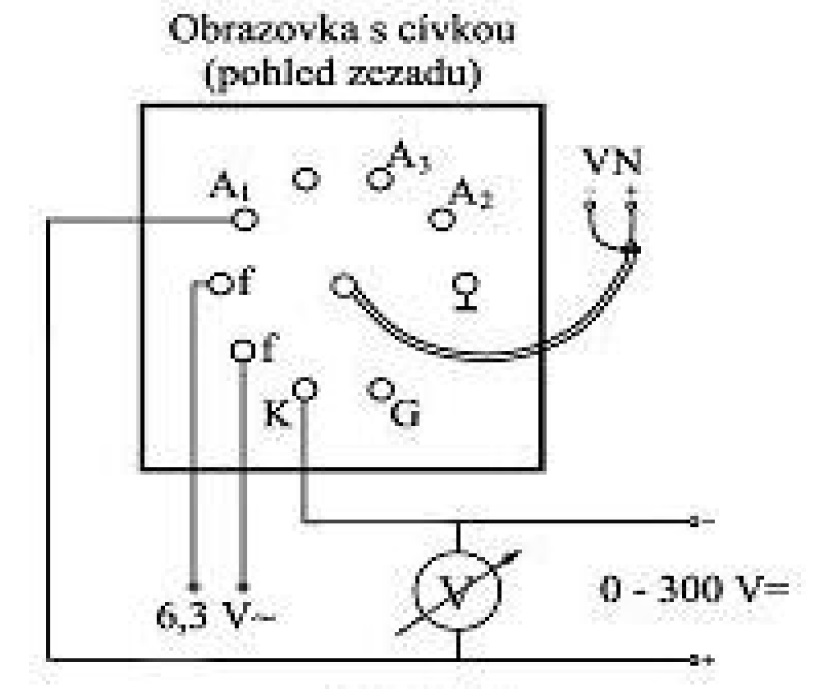
\includegraphics[width=7cm]{att/obrazek.jpg}
			\caption{Zapojení napájení obrazovky. Převzato z \cite{bib:zadani}.}
			\label{fig:obrazek}
			\end{figure}			
			
		\subsubsection{Měření $e/m$ v kolmém magnetickém poli}
			Při měření $e/m$ v kolmém magnetickém poli jsme sledovali závislost průměru kruhové dráhy svazku elektronů na proudu $I$ generujícím magnetické pole a na urychlovacím napětí $U$. Snažili jsme se volit hodnoty napětí a proudu tak, aby měření pokrývalo co největší rozsah, ale abychom zároveň byli ještě schopni změřit průměr kruhové dráhy svazku. 
			
	\subsection{Naměřené hodnoty}
		\subsubsection{Měření $e/m$ v podélném magnetickém poli}
			Naměřené a vypočítané hodnoty jsou uvedeny v Tab. \ref{tab:tab1}. Konstanty, kterých jsme užili k výpočtu dle teoretického úvodu, jsou zaznamenány v Tab. \ref{tab:konstanty}. Pomocné napětí jsme nastavili na $(140\pm1)$ V. Při tomto měření jsme finální hodnotu měrné hustoty náboje elektronu určili jako 
			\begin{equation}
				e/m = (1,970\pm0,007)~\mathrm{\cdot~10^{11}~C/kg}.
			\end{equation}

% Tabulka 1
\begin{table}[htbp]
  \centering  % Table generated by Excel2LaTeX from sheet 'List1'
% Table generated by Excel2LaTeX from sheet 'List1'
\begin{tabular}{|r|r|r|r|r|}
\hline
\boldmath{}\textbf{$U$ [kV]}\unboldmath{} & \boldmath{}\textbf{$I$ [A]}\unboldmath{} & \boldmath{}\textbf{$B$ [mT]}\unboldmath{} & \boldmath{}\textbf{$e/m~\mathrm{[10^{11}\cdot C/kg]}$}\unboldmath{} & \boldmath{}\textbf{$\sigma_{e/m}~\mathrm{[10^{11}\cdot C/kg]}$}\unboldmath{} \bigstrut\\
\hline
0,95  & 4,43  & 2,54  & 1,88  & 0,03 \bigstrut\\
\hline
0,97  & 4,48  & 2,57  & 1,87  & 0,03 \bigstrut\\
\hline
0,99  & 4,50  & 2,58  & 1,89  & 0,03 \bigstrut\\
\hline
1,01  & 4,50  & 2,58  & 1,93  & 0,03 \bigstrut\\
\hline
1,03  & 4,53  & 2,60  & 1,95  & 0,03 \bigstrut\\
\hline
1,05  & 4,55  & 2,61  & 1,96  & 0,03 \bigstrut\\
\hline
1,07  & 4,58  & 2,63  & 1,98  & 0,03 \bigstrut\\
\hline
1,09  & 4,60  & 2,64  & 1,99  & 0,03 \bigstrut\\
\hline
1,11  & 4,65  & 2,67  & 1,98  & 0,03 \bigstrut\\
\hline
1,13  & 4,68  & 2,68  & 2,00  & 0,03 \bigstrut\\
\hline
1,15  & 4,73  & 2,71  & 1,99  & 0,03 \bigstrut\\
\hline
1,17  & 4,75  & 2,73  & 2,01  & 0,03 \bigstrut\\
\hline
1,19  & 4,78  & 2,74  & 2,02  & 0,03 \bigstrut\\
\hline
1,21  & 4,83  & 2,77  & 2,01  & 0,03 \bigstrut\\
\hline
1,23  & 4,85  & 2,78  & 2,02  & 0,03 \bigstrut\\
\hline
1,25  & 4,90  & 2,81  & 2,01  & 0,03 \bigstrut\\
\hline
\multicolumn{3}{|r|}{\boldmath{}\textbf{$\overline{e/m}\pm\sigma_{\overline{e/m}}~\mathrm{[10^{11}\cdot C/kg]}$}\unboldmath{}} & \textbf{1,970} & \textbf{0,007} \bigstrut\\
\hline
\end{tabular}%

  
      \caption{Naměřené a vypočítané hodnoty pro výpočet $e/m$ pomocí podélného magnetického pole; $U$ je urychlovací napětí elektronu s chybou $0,1$ kV, $I$ proud na cívce s chybou $0,025$ A, $B$ magnetické pole, které tento proud generuje, s chybou $0,01$ mT (\ref{eq:chyba_neprime_mereni}), $e/m$, $\sigma_{e/m}$ měrná hustota náboje elektronu i se svou chybou, $\overline{e/m}$, $\sigma_{\overline{e/m}}$ pak její střední hodnota určená podle (\ref{eq:vazeny_prumer}) i s chybou (\ref{eq:chyba_vazeny_prumer}). }
      
  \label{tab:tab1}%
\end{table}%

		\subsubsection{Měření $e/m$ v kolmém magnetickém poli}
			Naměřené a vypočítané hodnoty jsou uvedeny v Tab. \ref{tab:tab2}. Konstanty, kterých jsme užili k výpočtu dle teoretického úvodu, jsou zaznamenány v Tab. \ref{tab:konstanty}. Při tomto měření jsme finální hodnotu měrné hustoty náboje elektronu určili jako 
			\begin{equation}
				e/m = (1,93\pm0,01)~\mathrm{\cdot~10^{11}~C/kg}.
			\end{equation}	

% Tabulka 2
\begin{table}[htbp]
\catcode`\-=12 % HAX na enable cline v českym bable
  \centering
  % Table generated by Excel2LaTeX from sheet 'List2'
  \begin{tabular}{|r|r|r|r|r|r|r|}
  \hline
  \boldmath{}\textbf{$U$ [V]}\unboldmath{} & \boldmath{}\textbf{$I$ [A]}\unboldmath{} & \boldmath{}\textbf{$d_1$ [cm]}\unboldmath{} & \boldmath{}\textbf{$d_2$ [cm]}\unboldmath{} & \boldmath{}\textbf{$r$ [cm]}\unboldmath{} & \boldmath{}\textbf{$e/m~\mathrm{[10^{11}\cdot C/kg]}$}\unboldmath{} & \boldmath{}\textbf{$\sigma_{e/m}~\mathrm{[10^{11}\cdot C/kg]}$}\unboldmath{} \bigstrut\\
  \hline
  120   & 1,6   & 15,45 & 9,70  & 2,9   & 1,98  & 0,05 \bigstrut\\
  \hline
  140   & 1,5   & 15,85 & 9,50  & 3,2   & 1,96  & 0,05 \bigstrut\\
  \hline
  178   & 1,5   & 16,70 & 9,90  & 3,4   & 2,24  & 0,05 \bigstrut\\
  \hline
  229   & 1,5   & 17,85 & 9,65  & 4,1   & 1,99  & 0,04 \bigstrut\\
  \hline
  79    & 1,7   & 14,55 & 9,70  & 2,4   & 1,62  & 0,05 \bigstrut\\
  \hline
  147   & 1,7   & 15,90 & 9,80  & 3,1   & 1,85  & 0,04 \bigstrut\\
  \hline
  202   & 1,7   & 17,00 & 9,80  & 3,6   & 1,82  & 0,04 \bigstrut\\
  \hline
  229   & 1,7   & 17,40 & 9,80  & 3,8   & 1,91  & 0,04 \bigstrut\\
  \hline
  120   & 2,1   & 14,50 & 9,40  & 2,6   & 1,41  & 0,04 \bigstrut\\
  \hline
  161   & 2,1   & 15,10 & 9,40  & 2,9   & 1,51  & 0,04 \bigstrut\\
  \hline
  202   & 2,1   & 15,40 & 9,40  & 3,0   & 1,75  & 0,04 \bigstrut\\
  \hline
  240   & 2,1   & 15,90 & 9,25  & 3,3   & 1,65  & 0,04 \bigstrut\\
  \hline
  153   & 1,2   & 17,20 & 10,00 & 3,6   & 2,69  & 0,06 \bigstrut\\
  \hline
  192   & 1,2   & 18,15 & 10,25 & 4,0   & 2,80  & 0,05 \bigstrut\\
  \hline
  234   & 1,2   & 19,25 & 10,90 & 4,2   & 3,06  & 0,05 \bigstrut\\
  \hline
  \multicolumn{1}{r|}{} & \multicolumn{4}{r|}{\boldmath{}\textbf{$\overline{e/m}\pm\sigma_{\overline{e/m}}~\mathrm{[10^{11}\cdot C/kg]}$}\unboldmath{}} & \textbf{1,93} & \textbf{0,01} \bigstrut\\
  \cline{2-7}\end{tabular}%
  
  
  \caption{Naměřené a vypočítané hodnoty pro výpočet $e/m$ pomocí kolmého magnetického pole; $U$ je urychlovací napětí elektronu s chybou $1$ V, $I$ proud na cívce s chybou $0,025$ A, $d_1$ a $d_2$ pozice měřítka kolem dráhy s chybou $0,05$ cm, $r$ z nich spočítaný poloměr kruhové dráhy svazku elektronů s chybou $0,04$~cm spočítanou podle (\ref{eq:chyba_neprime_mereni}), $e/m$, $\sigma_{e/m}$ měrná hustota náboje elektronu i se svou chybou, $\overline{e/m}$, $\sigma_{\overline{e/m}}$ pak její střední hodnota určená podle (\ref{eq:vazeny_prumer}) i s chybou (\ref{eq:chyba_vazeny_prumer}).}
  \label{tab:tab2}%
\end{table}%

% Tabulka konstant
\begin{table}[htbp]
\catcode`\-=12 % HAX na enable cline v českym bable
  \centering
\begin{tabular}{rrrrrrrr}
\toprule
\boldmath{}\textbf{$\mu_0~\mathrm{[Wb\cdot A^{-1}\cdot m^{-1}]}$}\unboldmath{} & \boldmath{}\textbf{$N$ [-]}\unboldmath{} & \boldmath{}\textbf{$l'$ [m]}\unboldmath{} & \boldmath{}\textbf{$l$ [m]}\unboldmath{} & \boldmath{}\textbf{$2a$ [m]}\unboldmath{} & \boldmath{}\textbf{$R$ [m]}\unboldmath{} & \boldmath{}\textbf{$k~\mathrm{[T\cdot A^{-1}]}$}\unboldmath{} & \boldmath{}\textbf{$N_H$ [-]}\unboldmath{} \\
\midrule
$1,257\cdot 10^{-6}$ & $174$ & $0,381$ & $0,249$ & $0,15$ & $0,15$ & $0,781\cdot 10^{-3}$ & $130$ \\
\bottomrule
\end{tabular}%

  \caption{Konstanty použité při výpočtech; $\mu_0$ je permeabilita vakua, $N$ počet závitů cívky, $l'$ délka cívky, $l$ délka obrazovky, $2a$ vzdálenost cívek, $R$ jejich střední poloměr, $k$ konstanta pro převod závislosti z $B$ na $I$ (viz (\ref{eq:B_to_I})) a $N_H$ počet závitů jedné Helmholtzovy cívky. }
  \label{tab:konstanty}%
\end{table}%
		
	\subsection{Diskuse}
		Námi změřené hodnoty $e/m$, tedy $(1,970\pm0,007)$ a $(1,93\pm0,01)~\mathrm{\cdot~10^{11}~C/kg}$ jsou větší, než je tabulková \cite{bib:tabulky} hodnota $1,759~\cdot~10^{11}~\mathrm{C/kg}$. Tento rozdíl nejspíš nebyl způsoben neuvažováním relativistických jevů, vzhledem k tomu, že je náš odhad chyby měření mnohem větší, než případný vliv těchto úvah. U obou dvou měření však můžeme mluvit o systematické chybě. 
		
		První měření bylo přesnější než druhé (nejen vzhledem k velikosti chyby závěrečné hodnoty, ale také metodou), ale určení momentu, kdy byla tečka na obrazovce nejostřejší, bylo značně subjektivní. Snažili jsme se ho tedy určovat alespoň co nejkonzistentněji, což by mělo teoreticky vést pouze k posunutí všech hodnot o stejnou konstantu. Dalším možným zdrojem rozdílu je použití vzorce pro $B$, který je pouze aproximací reálného chování v cívce. Během experimentu jsme také pozorovali kolísání napětí, což ale pravděpodobně nemělo výrazný vliv na výsledky.
		
		Druhé měření jsme měli lehce komplikovanější, vzhledem k tomu, že kolečko pro regulaci proudu na zdroji nefungovalo, jak mělo. Museli jsme tedy použít zdroj z jiné úlohy. Toto měření bylo o mnoho nepřesnější než to první, převážně vzhledem k nepřesnému měření poloměru kruhové dráhy svazku elektronů. U naměřených hodnot uvádíme v celém protokolu chyby rovné polovině nejmenšího dílku použitého měřítka, ale v tomto případě je jasné, že reálná chyba poloměru je minimálně o řád vyšší. Pozorující se mohl volně rozhodnout, co nazve momentem, kdy je dráha sevřena měřítkem, a ovlivnit tak finální hodnotu v řádu desítek procent. I toto měření jsme se snažili měřit alespoň konzistentně. Dalším zdrojem chyb mohlo být křivě umístěné měřítko za skleněnou baňkou. Naměřit více hodnot by nám k lepšímu výsledku pravděpodobně nepomohlo a těžko říct, jestli se dá poloměr dráhy ve skleněné kulaté baňce měřit lépe, než jak je aktuálně sestavena aparatura. 
		
		Námi naměřené hodnoty tedy se zmíněnými chybovými intervaly neodpovídají hodnotě tabulkové. Vezmeme-li však v potaz odhad reálné chyby obou měření, můžeme s jistotou říci, že jsme tabulkovou hodnotu nevyloučili. Měření nám dalo nahlédnout do chování elektronů v magnetickém poli a velmi pěkně demonstrovalo změnu tvarů při natáčení trubice v magnetickém poli (z kruhu na spirálu a přímku, viz příloha).
		
\section{Závěr}
	Sestavili jsme úlohu pro měření $e/m$ fokusací podélným magnetickým polem a provedli jsme měření pro několik různých hodnot urychlovacího napětí $U$ v rozmezí 950 -- 1250 V. 
	
	Změřili jsme měrný náboj elektronu $e/m$ ze zakřivení dráhy elektronů v kolmém magnetickém poli. Měření jsme provedli pro několik dvojic urychlovacího napětí a magnetizačního proudu. Vypočítali jsme příslušné hodnoty měrného náboje a z nich jsme určili střední hodnotu. 
	
	Otáčeli jsme katodovou trubicí sem a tam vůči magnetickému poli a sledovali jsme změnu trajektorie proudu elektronů. Viděli jsme, že z kruhového tvaru přecházela trajektorie na spirálovitý a nakonec se změnila v přímku. Pozorované dráhy jsme nakreslili do protokolu (viz příloha). 
	
\section {Použitá literatura}
% --- Literatura a reference -------------------------------------------
\begingroup
\renewcommand{\section}[2]{}

\begin{thebibliography}{9}
\bibitem{bib:zadani} Kolektiv KF, \emph{Návod k úloze: Měření měrného náboje elektronu} [Online], [cit. \today] \newline http://praktikum.fjfi.cvut.cz/pluginfile.php/425/mod\_resource/content/1/12a-edm.pdf

%\bibitem{bib:h3} Petr Chaloupka, \emph{Jak zpracovávat data} [Online], [cit. \today] \newline  https://dl.dropboxusercontent.com/u/11296940/zfm/h3.pdf

%\bibitem{bib:navody} Kolektiv KF, \emph{Návody k přístrojům} [Online], [cit. \today] \newline http://praktikum.fjfi.cvut.cz/documents/chybynav/navody-o.pdf

\bibitem{bib:chyby} Kolektiv KF, \emph{Chyby měření} [Online], [cit. \today] \newline http://praktikum.fjfi.cvut.cz/documents/chybynav/chyby-o.pdf

%\bibitem{bib:ctverce} Kolektiv KACH UPOL, \emph{Hodnocení analytických výsledků} [Online], [cit. \today] \newline http://ach.upol.cz/ucebnice/hodnoceni7.htm

\bibitem{bib:tabulky} J. Mikulčák a kol., Matematické, fyzikální a chemické tabulky \& vzorce. Prometheus,Praha 2009.\newline ISBN 978-80-7196-264-9

%\bibitem{bib:repo} Kolektiv autorů, \emph{Repozitář zdrojů k praktiku} [Online], [cit. \today] \newline  http://github.com/roesel/praktika

\end{thebibliography}
\endgroup
% ----------------------------------------------------------------------
\setcounter{equation}{0}
\numberwithin{equation}{section}
\clearpage
\part*{Přílohy}

\section{Domácí příprava}
	Domácí příprava je přiložena k protokolu spolu s nákresy trajektorií ze třetího úkolu.
%\clearpage
\section{Statistické zpracování dat}

%	Pro statistické zpracování využíváme aritmetického průměru:
%	\begin{equation} \label{eq:aritmeticky_prumer}
%	\overline{x} = \frac{1}{n}\sum\limits_{i=1}^{n}x_i,
%	\end{equation}
%
%	jehož směrodatnou odchylku spočítáme jako 
%	\begin{equation} \label{eq:smodch_aritmetickeho_prumeru}
%	\sigma_0 = \sqrt{\frac{1}{n} \sum\limits_{i=1}^{n}\left( x_i - \overline{x} \right)^2 },
%	\end{equation}
%	
%	kde $ x_i $ jsou jednotlivé naměřené hodnoty, $ n $ je počet měření, $ \overline{x} $ aritmetický průměr a $ \sigma_0 $ jeho chyba \cite{bib:chyby}.
%
%
%	jehož chybu spočítáme jako 
%	\begin{equation} \label{eq:chyba_aritmetickeho_prumeru}
%	\sigma_0 = \sqrt{\frac{1}{n(n-1)} \sum\limits_{i=1}^{n}\left( x_i - \overline{x} \right)^2 },
%	\end{equation}
%	
%	kde $ x_i $ jsou jednotlivé naměřené hodnoty, $ n $ je počet měření, $ \overline{x} $ aritmetický průměr a $ \sigma_0 $ jeho chyba \cite{bib:chyby}.
%	
Při nepřímém měření počítáme hodnotu s chybou dle následujících vztahů:
	\begin{equation}
	u = f(x, y, z, \ldots),
	\end{equation}
	\begin{displaymath}
	x = (\overline{x} \pm \sigma_x), \qquad
	y = (\overline{y} \pm \sigma_y), \qquad
	z = (\overline{z} \pm \sigma_z), \qquad
	\ldots,
	\end{displaymath}
	
	kde $ u $ je veličina, kterou určujeme nepřímo z měřených veličin $ x, y, z, \ldots $ 
	
	Pak
	\begin{displaymath}
	\overline{u} = f(\overline{x}, \overline{y}, \overline{z}, \ldots),
	\end{displaymath}
	\begin{equation}\label{eq:chyba_neprime_mereni}
	\sigma_u = \sqrt{\left( \frac{\partial f}{\partial x} \right)^2 \sigma^2_x + \left( \frac{\partial f}{\partial y} \right)^2 \sigma^2_y + \left( \frac{\partial f}{\partial z} \right)^2 \sigma^2_z + \ldots},
	\end{equation}
	\begin{displaymath}
	u = (\overline{u} \pm \sigma_ u).
	\end{displaymath}

V případě, že máme několik různě přesných měření stejné veličiny, používáme vztah pro vážený průměr:
	\begin{equation} 
	\label{eq:vazeny_prumer}
	\overline{x}=\frac{\sum\limits_{i=1}^{n}p_{i}x_{i}}{\sum\limits_{i=1}^{n}p_{i}},
	\end{equation}
	
	kde $\overline{x}$ je vážený průměr, $x_{i}$ jsou jednotlivá měření a pro $p_{i}$ platí
	 
	\begin{equation}
	p_{i}=\frac{1}{\sigma_{i}^{2}},
	\end{equation}
	
	kde $\sigma_{i}$ jsou jednotlivé chyby daných měření.
	 
	Celkovou chybu tedy vypočítáme ze vztahu
	\begin{equation} \label{eq:chyba_vazeny_prumer}
	\sigma_{0}=\sqrt{\frac{1}{\sum\limits_{i=1}^{n}p_{i}}}.
	\end{equation}
%
%\subsubsection{Metoda nejmenších čtverců}
%Snažíme-li se metodou nejmenších čtverců proložit data lineární závislostí $Y_i = ax_i+b$, dosazujeme hodnoty $x_i, y_i$ a snažíme se najít parametry $a$ a $b$ tak, aby byl součet všech kvadratických odchylek $\Delta Y_i^2$ minimální. Toho dosáhneme pomocí následujících vzorců \cite{bib:ctverce} :
%\begin{equation}\label{eq:ctverce_a}
%		a = \frac{n\sum\limits_{i=1}^{n}{x_i y_i}  - \sum\limits_{i=1}^{n}{x_i}\sum\limits_{i=1}^{n}{y_i}}{n\sum\limits_{i=1}^{n}{x_i^2}  - \left(\sum\limits_{i=1}^{n}{x_i}\right)^2}, \qquad \qquad
%		\sigma_a = \sqrt{\frac{n\sum\limits_{i=1}^{n}{(y_i - Y_i)^2} }{(n-2)\left(\sum\limits_{i=1}^{n}{x_i^2}  - \left(\sum\limits_{i=1}^{n}{x_i}\right)^2\right)}},
%\end{equation}
%
%\begin{equation}\label{eq:ctverce_b}
%		b = \frac{\sum\limits_{i=1}^{n}{x_i^2} \sum\limits_{i=1}^{n}{y_i}  - \sum\limits_{i=1}^{n}{x_i}\sum\limits_{i=1}^{n}{x_i y_i}}{n\sum\limits_{i=1}^{n}{x_i^2}  - \left(\sum\limits_{i=1}^{n}{x_i}\right)^2}, \qquad \qquad
%		\sigma_b = \sqrt{\frac{\sum\limits_{i=1}^{n}{x_i^2}\sum\limits_{i=1}^{n}{(y_i - Y_i)^2} }{n(n-2)\left(\sum\limits_{i=1}^{n}{x_i^2}  - \left(\sum\limits_{i=1}^{n}{x_i}\right)^2\right)}}.
%\end{equation}
%\section{Nákresy a schémata}
%			\begin{figure}[h!]
%			\centering
%			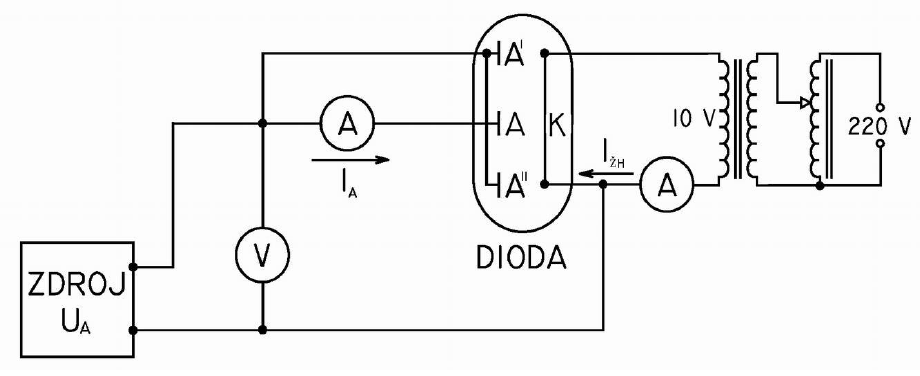
\includegraphics[width=12cm]{att/pyromet2.png}
%			\caption{Zapojení pro měření náběhového proudu. Převzato z \cite{bib:zadani}.}
%			\label{fig:s_aparatura_nasyc}
%			\end{figure}	
%			
%			
%\clearpage
%\section{Tabulky a grafy}
%\catcode`\-=12 % HAX na enable cline v českym bable
%
%
%	\begin{figure}[h!]
%	\begin{center}
%	    \vspace*{-1cm}
%		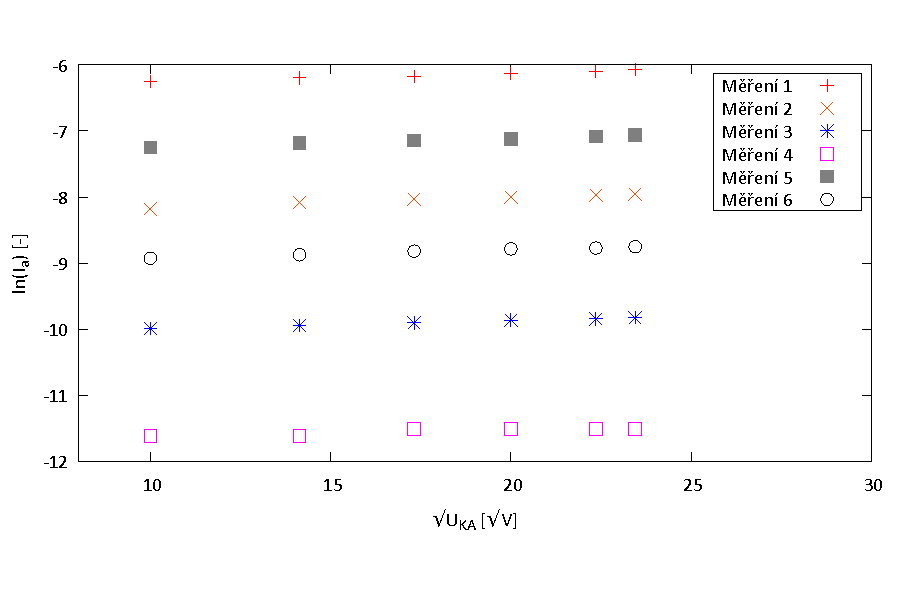
\includegraphics[width=\linewidth]{../gnuplot/termise.pdf}
%	    \vspace*{-2cm}
%		\caption{Měření nasyceného proudu; závislost celkového proudu $I_a$ (resp. jeho logaritmu) na napětí mezi katodou a anodou $U_{KA}$ (resp. jeho odmocnině).} 
%		\label{fig:g_termise}
%	\end{center}
%	\end{figure}		
%		
%\clearpage
% --- Konec dokumentu --------------------------------------------------


\end{document}

